% 图 8.14 XY 模型单涡旋：13x13 格点上面内磁矩绕涡旋心连续旋转 2π
\documentclass[tikz,border=5pt]{standalone}
\usetikzlibrary{arrows.meta}
\usepackage{amsmath}
\usepackage{bm}
\usepackage{fontspec}
\setmainfont{Times New Roman}
\begin{document}
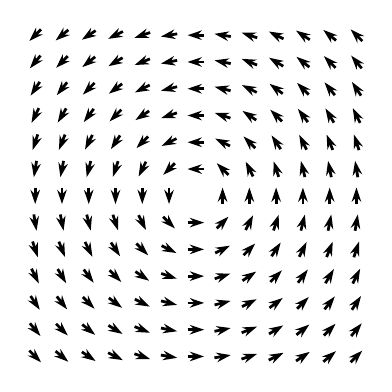
\begin{tikzpicture}[line width=0.8pt,>=Stealth]
\def\s{0.34}   % lattice spacing
\def\l{0.21}   % arrow length
\foreach \i in {0,...,12}{
  \foreach \j in {0,...,12}{
    \pgfmathsetmacro{\x}{(\i-6)*\s}
    \pgfmathsetmacro{\y}{(\j-6)*\s}
    \pgfmathsetmacro{\r}{sqrt(\x*\x+\y*\y)}
    \ifdim\r pt>0.02pt
      \pgfmathsetmacro{\a}{atan2(\y,\x)+90}
      \draw[->,line width=1.0,-{Stealth[length=1.8mm,width=1.2mm]}]
        ({\x-0.5*\l*cos(\a)},{\y-0.5*\l*sin(\a)})
        -- ({\x+0.5*\l*cos(\a)},{\y+0.5*\l*sin(\a)});
    \fi
}}
\end{tikzpicture}
\end{document}
